\section{Abalone Exploratory Analysis}

\subsection{Missing Data}

I first looked for any missing data that may be in the abalone dataset. Once the data was in a dataframe I checked the dtypes of each column. Curiously the Rings column is displayed as an object type, when it should be numerical. I was able to coerce the Rings column to a numerical type by converting it with pandas and ignoring all rows that could not be converted. Every column except the Sex column is now a float64 type.
 
Next I scanned the entire dataframe for NaN values.

\begin{figure}[H]
  \centering
  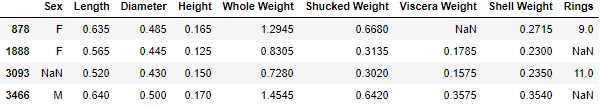
\includegraphics[scale=0.5,width=100mm]{./images/abalone-nan.png}
  \caption{Searching for NaN values within the abalone dataset}
  \label{fig:abalones-nan}
\end{figure}

In figure \ref{fig:abalones-nan} we can see that there are 4 rows with NaN values. This could have been the result of some invalid data gathering, or some computational error. Either way the Viscera Weight on row 878, the Rings on row 1888, the Sex on row 3093 and again the Rings on row 3466 are invalid so they needed to be removed as there is a high probability they might throw our regressions off later on.

\subsection{Erroneous Data}

\begin{figure}[H]
  \centering
  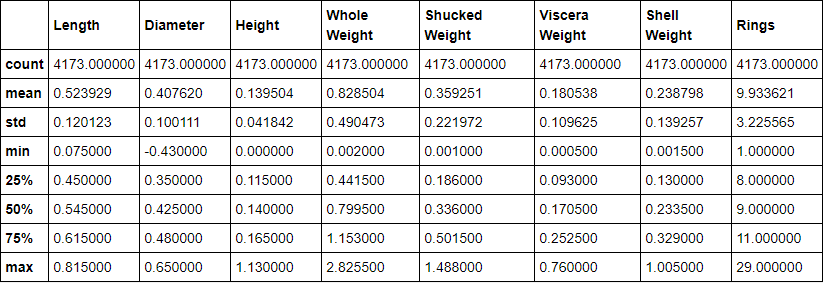
\includegraphics[scale=0.5,width=100mm]{./images/abalone-df-describe.png}
  \caption{Summary of abalone dataset}
  \label{fig:abalones-df-describe}
\end{figure}

Figure \ref{fig:abalones-df-describe} shows a complete summary of the data contained within the abalone dataset. Looking at this summary I noted a few oddities. Height has a minimum value of zero, this should not be possible as even infant abalones must have some height above zero. Diameter is showing a min value of a minus number, this again should not be possible.

\begin{figure}[H]
  \centering
  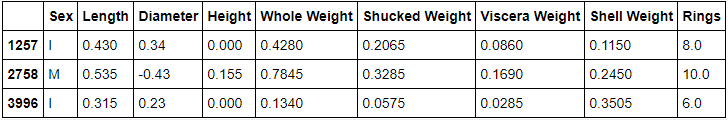
\includegraphics[scale=0.5,width=100mm]{./images/abalone-less-than-zero.png}
  \caption{Values less than or equal to zero}
  \label{fig:abalones-less-than-zero}
\end{figure}

Figure \ref{fig:abalones-less-than-zero} shows rows that have less than or equal to zero values. As explained above these rows are erroneous. There are a few things we could do with these rows. We could replace the erroneous values with the mean value of the entire column. For example in the case of the Height column we could get the mean of the Height column and replace the zero with that value. Alternatively we can just drop the rows completely As there are only 3 rows detected as erroneous it seems reasonable to simply drop them for now.

I found the shucked weight column interesting. It is described as weight without the shell. If this is the case than it would be interesting to see if there are any abalones whose whole weight is less than their shucked weight.

\begin{figure}[H]
  \centering
  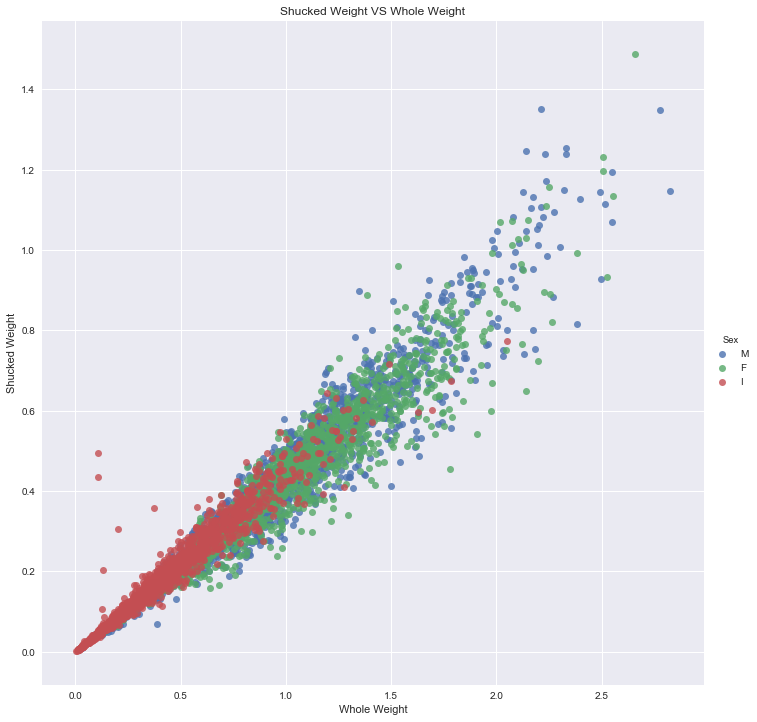
\includegraphics[scale=0.5,width=100mm]{./images/abalone-shucked-weight-vs-whole.png}
  \caption{Shucked Weight vs Whole Weight broken down by Sex}
  \label{fig:shucked-vs-whole}
\end{figure}

Figure \ref{fig:shucked-vs-whole} shows a scatter plot of shucked weight versus whole weight. Most of the data does seems to follow a pretty linear pattern, however notice in the bottom left there are a few outliers with of infant type whose shucked weight is greater than the whole weight. Figure \ref{fig:shucked-greater-than-whole} shows the 4 rows with the offending data. For the purposes of this analysis I chose to drop those rows

\begin{figure}[H]
  \centering
  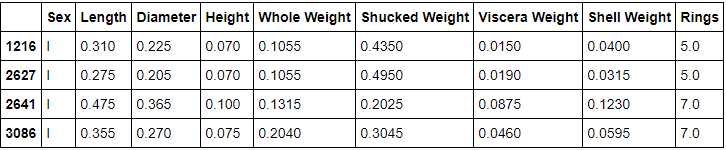
\includegraphics[scale=0.5,width=100mm]{./images/abalone-shucked-greater-than-whole.png}
  \caption{Shucked Weight greater than Whole Weight}
  \label{fig:shucked-greater-than-whole}
\end{figure}

